\section{Examples and performance benchmarks}
\label{sec:results}

We demonstrate the effectiveness of our preconditioner through several examples.
Figure~\ref{fig:DD-teaser} illustrates two smoke simulations with more than one billion of active degrees of freedom, each. 
Figure~\ref{fig:flasks} shows a network of interconnected vessels where smoke enters from the lower
left corner and exists from the upper right corner. Our solver is able to
capture the correct incompressible behavior in relatively few iterations with
four subdomains.  Figure~\ref{fig:free-surface-flow} shows an example where
water is poured in a pool with multiple immersed objects, creating complex
Neumann interfaces. Figure~\ref{fig:snake-channel} shows an example where water flows in
a channel with multiple interior walls, which cause the flow to meander around
them. Figure~\ref{fig:performance-results} provides a breakdown of individual kernels of our Schur Complement solver for all these examples, along with timings for alternative
solvers, detailed in the following section.\added{ We note that no vorticity confinement was used in our smoke examples. Finally, in the interest of efficiency we used as high of a
  CFL number as our examples could tolerate -- sometimes leading to minor loss of detail}.


\section{Discussion}
\label{sec:discussion}

\paragraph{Evaluation of convergence and scaling}

In our benchmarks, we compared the convergence behavior of our Schur-Complement Domain Decomposition preconditioned CG \emph{(``DDPCG'')} with a standard Incomplete Cholesky
preconditioner \emph{(``ICPCG'')} \cite{Foster:2001:PAO}, and a standard Multigrid-Preconditioned CG algorithm \emph{(``MGPCG'')} \cite{mcadams2010parallel}. For
the multigrid option, specifically, we note that although we did not experiment with improved CPU-based versions of MGPCG that take extra steps to better capture the topology of
the domain on coarser levels of the multigrid hierarchy \cite{Westermann:2014:LiquidAdaptiveHexahedral}, we invested a significant effort to optimize the stock MGPCG to the
absolute best of our capacity, both on the CPU as well as on the accelerator cards  -- this was a natural
step to take, as the multigrid kernels used in MGPCG are re-used in the subdomain solver of our own DDPCG method. We produced two, heavily optimized MGPCG implementations:
One designed to run exclusively on the CPU, and one designed to run \emph{homogeneously} 
on just a single GPU, for problems that are small enough to fit entirely in GPU memory. There is only one algorithmic difference between the two implementations: The pure-CPU MGPCG
was set up to solve the coarsest level of the multigrid hierarchy using ICPCG -- this was done to improve the convergence behavior at the bottom of the multigrid cycle, which
was crucial in obtaining acceptable performance at our examples with more than a billion degrees of freedom (without requiring an extremely deep, and occasionally inaccurate
V-cycle). The GPU-native implementation of MGPCG used a large number of smoother applications at the bottom of the V-cycle (which was effective for its smaller problem size), to
avoid using Incomplete Cholesky on the GPU. We benchmarked the pure-CPU MGPCG solver on the faster (dual socket) of our two test platforms.

In all our examples, the ICPCG solver exhibited dramatically slower convergence performance than both MGPCG, and our proposed DDPCG method, often needing more than an order of
magnitude of iterations higher than DDPCG to reach comparable performance. We were unable to use ICPCG for our largest of examples with billions of cells, as the footprint of the
explicitly constructed matrices would cause it to run out of memory. For our smallest examples, even each iteration of our heterogeneous DDPCG actually required less time than one
CPU-based ICPCG iteration. As a consequence, we did not find ICPCG to be a competitive alternative. 

On the other hand, the convergence behavior of MGPCG remained competitive in several of our smaller-size examples. We should point out that the behavior of DDPCG is tunable;
investing more V-cycles in the independent subdomain solves, or additional multigrid iterations in the interface solve can boost its convergence efficiency. We found MGPCG to be
most competitive with our DDPCG technique in the context of our smaller examples, especially the free-surface water simulations. This is attributed to the prominence of Dirichlet
boundary conditions in those scenarios, which dramatically improves the efficacy of smoothing boundary regions, which is essential for multigrid to behave favorably as a
preconditioner \cite{mcadams2010parallel}. On average, across the various frames of the water simulations (Figures
\ref{fig:snake-channel},\ref{fig:free-surface-flow}) MGPCG would converge in no more than $1.5$x-$3$x the number of iterations required by our tuned DDPCG, while in the smoke
simulation of Figure \ref{fig:flasks}, MGPCG required approximately $2$x-$2.5$x more iterations than DDPCG. In terms of run time, however, the findings paint a quite different
picture. The smaller two of our examples (Figures \ref{fig:flasks}, \ref{fig:free-surface-flow}) were compact enough to fit on just a single GPU card, where a single iteration of MGPCG
was between $5$x-$8$x times faster than a DDPCG iteration. Thus, in spite of the moderately slower convergence of MGPCG, its faster per-iteration cost on the homogeneous,
single-GPU implementation makes it preferable to DDPCG by a factor of $3$x-$5$x. Incidentally, the geometry of the smoke example in Figure \ref{fig:flasks} led to another
interesting observation: Although the narrow cylindrical connectors between the glass spheres allowed for a small interface between subdomains used in our solver (and a
reduction in CPU computation cost), the same geometry traits increased the approximation error induced by our adaptive coarsening of the subdomain interiors, increasing the
required iterations for PCG convergence.

The situation is dramatically different for our larger simulation examples, which cannot be solved with MGPCG on a single accelerator card. For those examples, the only practical
alternative was to run MGPCG homogeneously on the CPU. In this context, we observed that each iteration of our DDPCG method was within $20\%$ of the cost of a CPU-only MGPCG
iteration. However, for the large-scale examples, dominated by Neumann boundary conditions, we observed MGPCG requiring up to $5$x more iterations for convergence, leading to a
$3.5$x-$4.5$x performance benefit of DDPCG versus the CPU-only MGPCG. We conclude that for small problem sizes, in the order of $100$M degrees of freedom or less, a
\emph{homogeneous GPU} implementation of MGPCG is the preferred solver, provided that the problem can fully fit in GPU memory. For problem sizes that do not fit completely in GPU
memory, DDPCG appears to be consistently superior to CPU-based MGPCG, with the performance gap becoming larger as the resolution increases.

\begin{figure}[t!]
\begin{center}
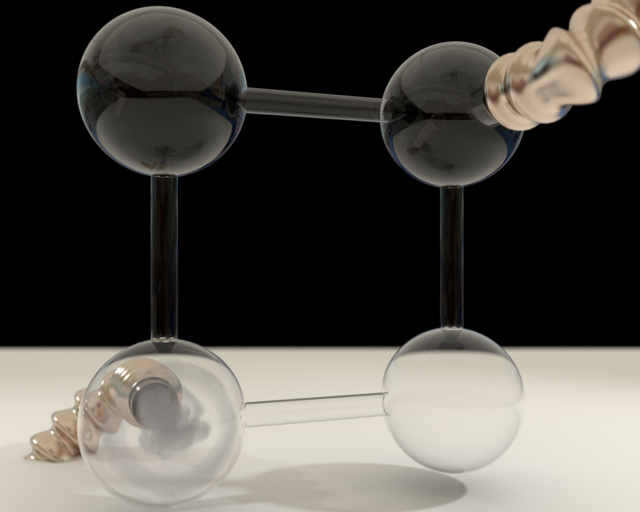
\includegraphics[width=.24\columnwidth]{images/DD/flasks_050.png} 
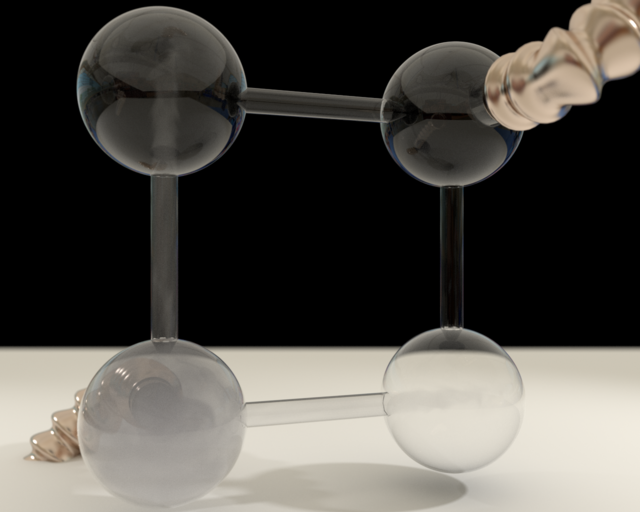
\includegraphics[width=.24\columnwidth]{images/DD/flasks_200.png} 
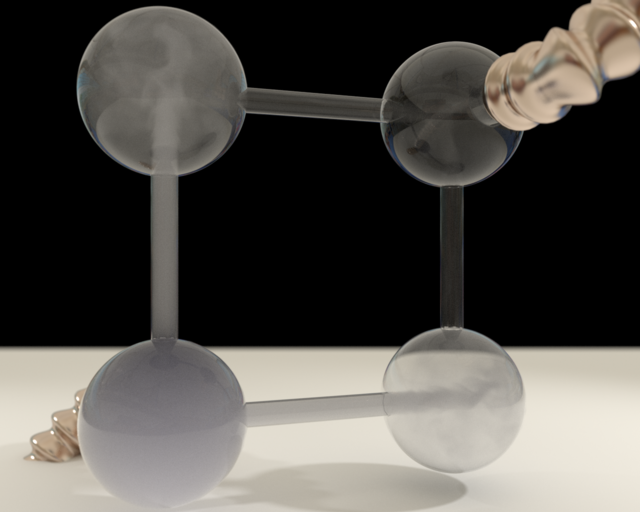
\includegraphics[width=.24\columnwidth]{images/DD/flasks_500.png} 
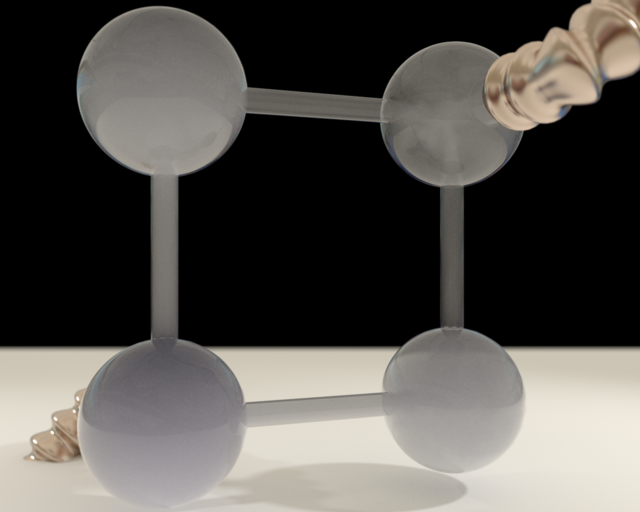
\includegraphics[width=.24\columnwidth]{images/DD/flasks_800.png} 
\end{center}
\caption{Smoke flow in a network of interconnected vessels simulated using a $1024^2 \times512$ background grid and $42$ million active cells. The computational domain was divided into four subdomains. The proper flux is observed both in the inlet and the outlet of the flow.}
\label{fig:flasks}
\end{figure}

\paragraph{Limitations and future work}

The most fundamental limitation of our proposed method is that, in order for its scaling benefits to take effect, it needs to be applied to a problem of adequately
large size. In designing our (GPU-hosted) multigrid cycle for the
solution of the subdomain problems, we made a conscious choice to keep the design of this solver as simple as possible, approximating the domain at voxel-accuracy at
every level, and not enacting any remedies for topological inconsistencies, such as regions merging or small Neumann gaps disappearing after coarsening. This was
done in the interest of simplicity, to facilitate low-level optimizations of the solver components. It is quite likely that topology-conscious coarsening schemes
\cite{Westermann:2014:LiquidAdaptiveHexahedral} could further improve the convergence properties of this component, and the balance between enacting such
improvements and retaining opportunities for aggressive optimization certainly merits investigation. Finally, one should not discount the software engineering
challenges that are still associated with developing numerical software that is as inherently heterogeneous as our solver. The established programming
paradigms that are available for \emph{homogeneous} thread-based parallel development (e.g. OpenMP) are arguably much more accessible to the non-expert
developer. Given the precedent of CUDA, and the growing presence of heterogeneity in modern systems, we hope that programming abstractions for these platforms
will continue to evolve. 

The scope of our work was specifically restricted to the design and optimization of the pressure Poisson solver on a heterogeneous computer. We also specifically targeted fluid
simulation on \emph{uniform} grids in the development of our solver. Although extending the concepts of our solver to an adaptive discretization is certainly possible from an
algebraic perspective, we feel that a careful investigation is warranted to make sure that 
the complexity of work that needs to happen on the interface region remains comparatively lower. This aspect, as well as practices for efficient dynamic partitioning
of temporally changing adaptive grids would be an exciting topic for continued investigation. 

A very interesting venue for future work might focus on extending our technique to deeper hierarchies of heterogeneous platforms, using for example clusters of
network-interconnected GPU-accelerated nodes. The same way that we used a multigrid cycle to approximate a subdomain solver, one could envision using our entire
preconditioner as the approximate solver for a subdomain assigned to each cluster node, which is internally subdivided to use GPU accelerations as we currently
do. Although bandwidths of network interconnects would be even slower than that of PCIe, due to economy of scale the relevant asymptotics (relative size of
interfaces vs. entire grid) could remain favorable. Finally, emerging GPU architectures and technologies (stacked memory, integration of CPU and GPU) might
facilitate programming in a homogeneous model (using capabilities such as unified memory spaces), but non-homogeneity in memory bandwidth is almost certain to
persist in some form (cores having significantly higher bandwidth to their ``local'' region of memory). We feel that the adaptation of solver concepts to such
architectural traits is an exciting research thread.

\begin{figure*}[t]
\begin{center}
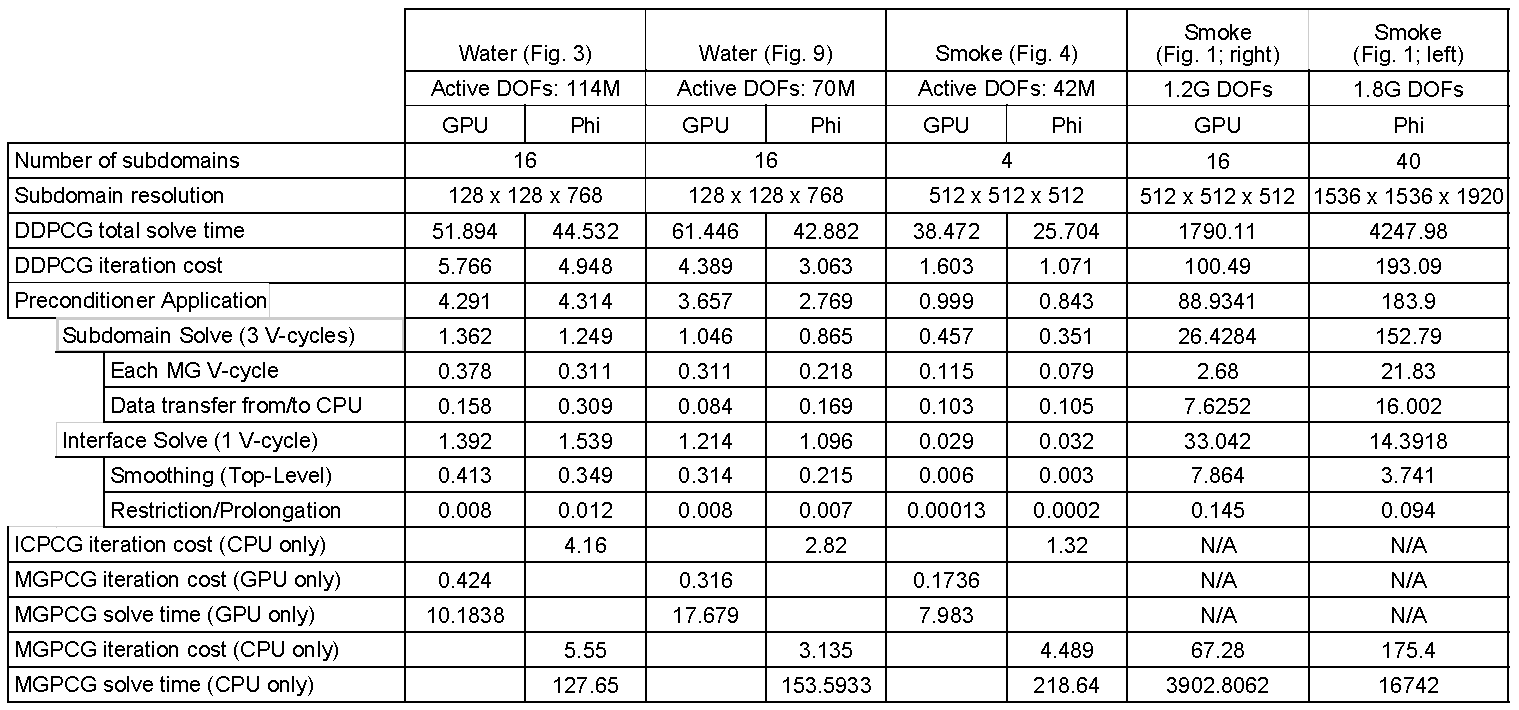
\includegraphics[width=.94\textwidth]{images/DD/performance_results.pdf}
\end{center}
\caption{Timing information for four examples. \textbf{All run times cited are in seconds}. Our ``GPU'' platform is an Intel Xeon
E5-1650v3 CPU equipped with two NVidia GTX Titan X GPUs and 128GB RAM, while our ``Phi'' platform is an Intel Xeon E5-2650v3 CPU equipped with six Intel Xeon Phi 31S1P cards.
\added{The row labeled \textsf{Preconditioner Application} reflects the preconditioning cost for a single PCG iteration.}
}
\label{fig:performance-results}
\end{figure*}

